\section{\methodname: An Effective RL Recipe for Code Localization}

This section presents the methodology used to train \methodname, covering training data curation and environment construction (\S\ref{sec:data_creation}), the agent scaffold (\S\ref{sec:agent_scaffold}), reward design (\S\ref{sec:reward_design}), and the RL training setup (\S\ref{sec:train_algo}). Figure~\ref{fig:system_diagram} provides an overview of our approach.

\begin{figure*}[!ht]
    \centering
    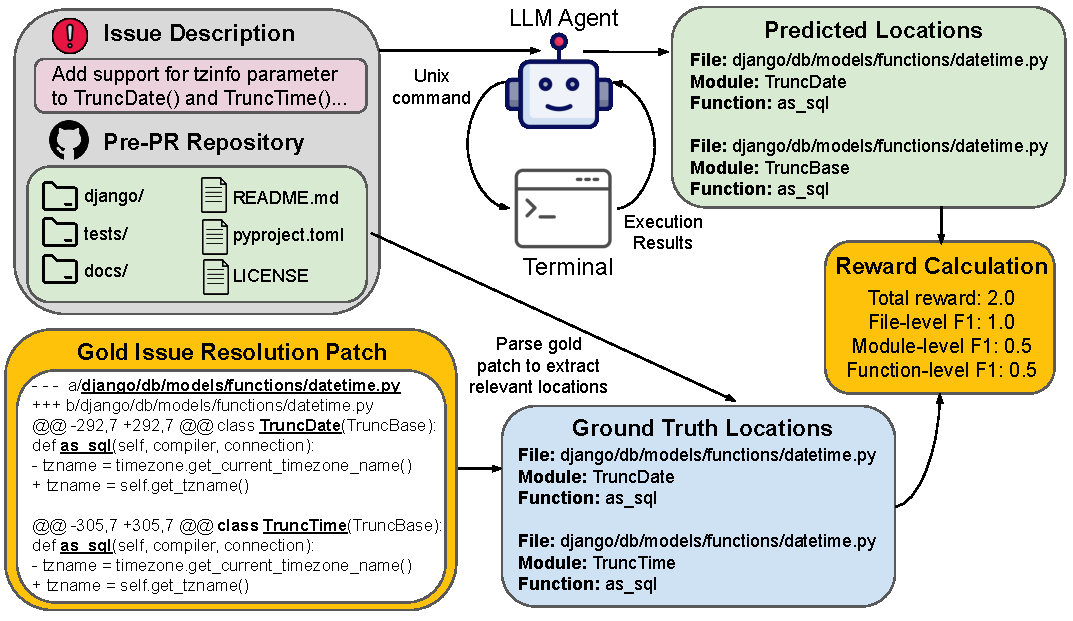
\includegraphics[width=0.7\textwidth]{COLM/Figures/sys_diagram_new_cropped (2).pdf}
    \caption{An overview of \methodname: given a GitHub issue, the LLM agent navigates the pre-PR codebase using a terminal and predicts the relevant set of files, modules, and functions. The reward function computes F1 scores for these three granularities using ground truth locations extracted from the gold issue resolution patch.}
    \label{fig:system_diagram}
\end{figure*}

\subsection{Data and Environment Curation}
\label{sec:data_creation}
Given a GitHub issue $\mathcal{I}$ in a Python repository $\mathcal{R}$, we process the ground-truth issue resolution patch $\mathcal{P}$ to extract the localization targets at three granularities. Specifically, we define the ground-truth target as $y^{\star} = (F^{\star}, M^{\star}, U^{\star})$, where $F^{\star} = {f_1^{\star}, \dots, f_{N_f}^{\star}}$ is the set of modified files, $M^{\star} = {m_1^{\star}, \dots, m_{N_m}^{\star}}$ is the set of modified modules, and $U^{\star} = {u_1^{\star}, \dots, u_{N_u}^{\star}}$ is the set of functions or methods edited by the patch $\mathcal{P}$. An example of these targets is illustrated in Figure~\ref{fig:system_diagram}. The LLM agent is tasked with predicting $y^{\star}$ given the issue description $\mathcal{I}$ and the pre-PR repository state $\mathcal{R}$. We extract ground truth by using patch-processing scripts from ~\citet{chen-etal-2025-locagent}.

We curate training instances by processing GitHub issues collected by prior work~\citep{yang2025swesmithscalingdatasoftware, pan2025trainingsoftwareengineeringagents}, originally intended for training agents to fix issues. We discard issues with empty descriptions and whose PRs create or delete files, as the agent cannot predict the name of newly created files and we cannot determine relevant modules or functions for deleted files. We ignore non-Python files (e.g., \texttt{README.md}) because function and module-level information cannot be extracted from them. We construct the RL environment by cloning the pre-PR commit of the repository to a specific path known to the agent via its prompt. As localization does not require code execution, we do not install dependencies or use sandboxes. Notably, as our agent only uses a terminal, its environment setup overhead is much lower than prior agents that use code graphs, vector indices, or dependency parsers.

\subsection{OpenHands-Bash: Our Agent Scaffold}\label{sec:agent_scaffold}

We use OpenHands Agent SDK~\citep{wang2025openhandssoftwareagentsdk} to implement our agent as it performs strongly across software engineering benchmarks, implements core tools (e.g., terminal), supports parallel tool-calling, and has a modular design that easily integrates with our training backend. The agent is equipped with a \texttt{Terminal} tool that supports standard Unix commands (e.g., \texttt{find}, \texttt{ls}, \texttt{sed}). We install \texttt{ripgrep}~\citep{ripgrep} in the agent's environment, which is a command-line utility for fast grep-style search using regex patterns recursively through all code files in a directory. Furthermore, the agent uses the \texttt{LocalizationFinish} tool to submit predictions. We refer to this scaffold as \textbf{OpenHands-Bash}.

Our initial experiments used a string-based output format from \citet{chen-etal-2025-locagent}, but we found training with this format is sensitive to noisy reward signals due to brittle validation and parsing. We address this by requiring the agent to terminate via the \texttt{LocalizationFinish} tool, enforcing a structured output schema and simplifying parsing, improving reward fidelity. Appendix~\ref{appendix:prompts} includes detailed prompts and tool definitions for our agent.

\subsection{Reward Design}\label{sec:reward_design}
For each trajectory $\tau$ sampled from the agent, we extract the prediction $y = (F, M, G)$ from the \texttt{LocalizationFinish} tool, which specifies the predicted files, modules, and functions. Given the ground-truth $y^{\star} = (F^{\star}, M^{\star}, G^{\star})$, we compute F1 scores at each granularity. For each set $S \in \{F, M, G\}$ with the corresponding ground truth set $S^{\star} \in \{F^{\star}, M^{\star}, G^{\star}\}$, we compute F1 score (i.e. harmonic mean of precision and recall): $r^{\mathsf{F1-file}}$, $r^{\mathsf{F1-module}}$, and $r^{\mathsf{F1-func}}$. Our reward function is defined as:
\begin{equation}
\begin{aligned}
    r(\tau, y, y^{\star}) &= r^{\mathsf{F1-file}}(y, y^{\star}) + r^{\mathsf{F1-module}}(y, y^{\star}) + r^{\mathsf{F1-func}}(y, y^{\star})
\end{aligned}
\label{eqn:reward}
\end{equation}
Earlier training runs for our 14B LLM collapse to near-zero rewards in later stages as the agent frequently exhausted the step budget without submitting its answer. We fix this with an auxiliary binary reward $r^{\mathsf{turn}}(\tau, k)$ that assigns 1 if and only if the agent terminates in exactly $k$ turns, where $k$ is the step limit. Thus, the reward for 14B LLM adds this binary term to $r(\tau, y, y^{\star})$ in Equation~\ref{eqn:reward}. Appendix~\ref{appendix:reward_function} includes more discussion on reward design.

\subsection{RL Training Algorithm}\label{sec:train_algo}

We use SkyRL~\citep{griggs2025skrylv01} and train asynchronously~\citep{fu2026areallargescaleasynchronousreinforcement} to improve GPU utilization by parallelizing rollouts and weight optimization and set maximum staleness to $t=4$. 
% After each optimization step, we update weights in the vLLM~\citep{kwon2023efficient} engines and terminate any incomplete inference requests.
We train models using Group Sequence Policy Optimization (GSPO)~\citep{zheng2025groupsequencepolicyoptimization}. Given model parameters $\theta$ ; $i$ indexes sequences in a group of size $G$; $y_i$ is the $i^{th}$ output sequence with length $|y_i|$, and $y_{i,t}$ is its $t^{th}$ token. $\pi_\theta$ and $\pi_{\theta_{\text{old}}}$ are current and older policies, $\hat{A}_i$ is the advantage, and $\varepsilon$ is the clipping parameter:
{
\small % or \footnotesize
\begin{align}
    \mathcal{J}_{\text{GSPO}}(\theta) &= 
    \mathbb{E}_i \left[ \frac{1}{G} \sum_{i=1}^{G} \min\left( s_i(\theta) \hat{A}_i,\, \text{clip}\left( s_i(\theta), 1-\varepsilon, 1+\varepsilon \right) \hat{A}_i \right) \right]
    \label{eq:gspo}
\end{align}
}
where,  $s_i$ is the importance ratio derived from sequence likelihood~\citep{zheng-etal-2023-click}:
\begin{align}
    s_i(\theta) = \exp\left( \frac{1}{|y_i|} \sum_{t=1}^{|y_i|} \log \frac{\pi_\theta(y_{i,t} | x, y_{i,<t})}{\pi_{\theta_{\text{old}}}(y_{i,t} | x, y_{i,<t})} \right)
    \label{eq:is}
\end{align}
Following ~\citet{liu2025understandingr1zeroliketrainingcritical}, we remove standard deviation from the advantage calculation.
\begin{align}
    \hat{A}_i = r_i - \text{mean}(\mathbf{r}), \mathbf{r} = \{r_1, ..., r_G\}
\end{align}
Finally, we remove KL regularization from the loss, disable entropy loss, and mask loss for rollouts that exhaust maximum steps without submitting predictions. Additional analysis on the effect of the RL algorithm on localization performance can be found in Appendix~\ref{appendix:rl_ablation_study}.